\documentclass[12pt]{article}
\usepackage[papersize={8cm,14cm},margin={.5cm,.5cm}]{geometry}
\usepackage{common}
\usepackage{amssymb}
\begin{document}
\begin{problem}
\item[2.] $\triangle{ABC}$ 中,$D$、$E$、$F$ 三點分別在 $\overline{BC}$、$\overline{AC}$、$\overline{AB}$ 上,如圖(二)所示。已知四邊形 $BDEF$ 是以 $\overline{DF}$ 為對稱軸的線對稱圖形,且四邊形 $CDFE$ 是以 $\overline{DE}$ 為對稱軸的線對稱圖形。若 $\angle{B} = 80^\circ$,則 $\angle{DFE}$ 的度數為何?
  \begin{figure}[ht]
    \centering
    \vspace*{-1ex}
    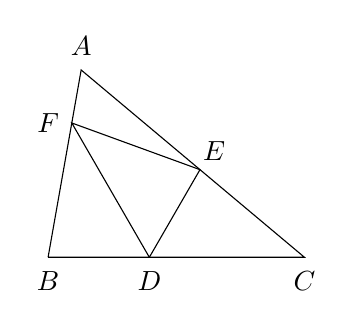
\begin{tikzpicture}
      \draw (-1.286,0) -- (1.97,0) -- (-.866,2.379) -- (-1.286,0);
      \draw (0,0) -- (-.985,1.706) -- (.643,1.113) -- (0,0);
      \node at (-.866,2.679) {$A$};
      \node at (-1.286,-.3) {$B$};
      \node at (1.97,-.3) {$C$};
      \node at (0,-.3) {$D$};
      \node at (.823,1.353) {$E$};
      \node at (-1.285,1.706) {$F$};
    \end{tikzpicture}
    \vspace*{-1ex}
    \caption*{圖(二)}
    \vspace*{-2ex}
  \end{figure}
  \begin{choices}
    \item $30$
    \item $35$
    \item $40$
    \item $45$
  \end{choices}
\end{problem}
\end{document}
